% 1956 年全国卷第 8 题：底面 ABCD 为菱形的四棱柱示意图。
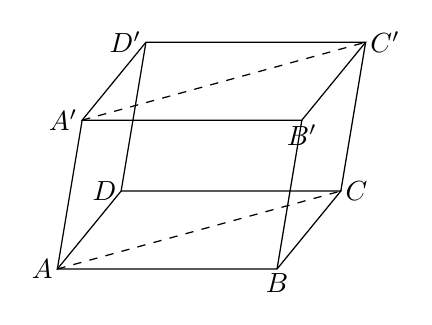
\begin{tikzpicture}[scale=0.9, line width=0.45pt,
  every node/.style={inner sep=1.5pt}]
  \coordinate (A) at (0,0);
  \coordinate (B) at (3.1,0);
  \coordinate (C) at (4.0,1.1);
  \coordinate (D) at (0.9,1.1);
  \coordinate (A1) at (0.35,2.1);
  \coordinate (B1) at (3.45,2.1);
  \coordinate (C1) at (4.35,3.2);
  \coordinate (D1) at (1.25,3.2);
  \draw (A)--(B)--(C)--(D)--cycle;
  \draw (A1)--(B1)--(C1)--(D1)--cycle;
  \draw (A)--(A1) (B)--(B1) (C)--(C1) (D)--(D1);
  \draw[dashed] (A)--(C) (A1)--(C1);
  \node[anchor=east] at (A) {$A$};
  \node[anchor=north] at (B) {$B$};
  \node[anchor=west] at (C) {$C$};
  \node[anchor=east] at (D) {$D$};
  \node[anchor=east] at (A1) {$A'$};
  \node[anchor=north] at (B1) {$B'$};
  \node[anchor=west] at (C1) {$C'$};
  \node[anchor=east] at (D1) {$D'$};
\end{tikzpicture}
